\chapter{Versuchsaufbau und -durchf�hrung}
\section{Dopplerspektroskopie}

\begin{figure}[ht]
 \center
  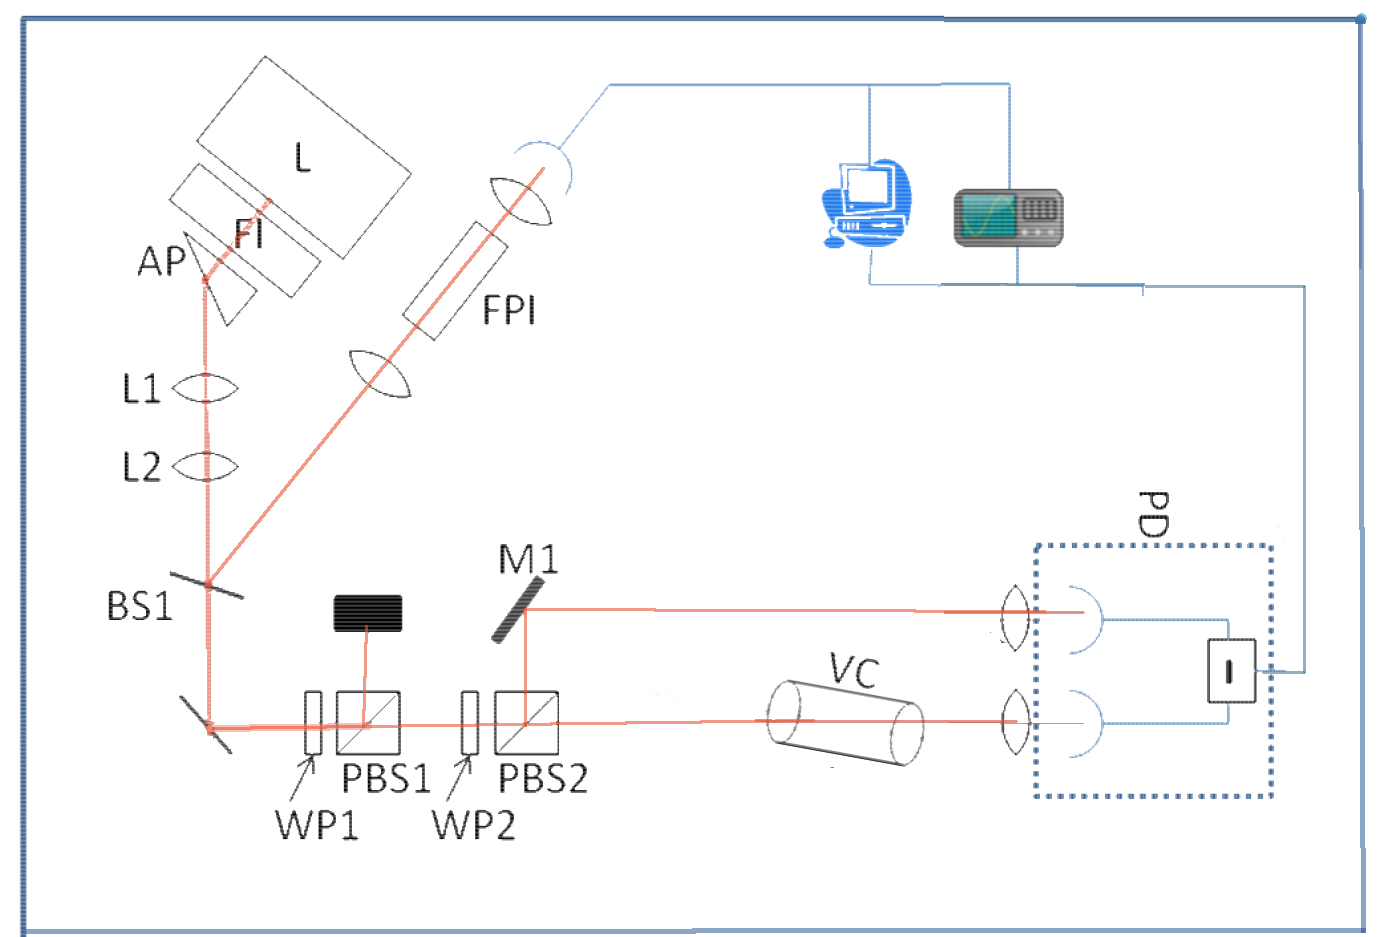
\includegraphics[width=0.85\textwidth]{./aufbau.png}
  \caption{Schematischer Aufbau Dopplerspektroskopie}
\end{figure}
Der Laserstrahl trifft durch eine Faraday-Diode (FI) auf ein Prisma (AP), welches die elliptische Strahlform korrigiert. 

Die Faraday-Diode soll R�ckreflexionen auf die Laserquelle blockieren, um daraus resultierende St�rquellen zu vermeiden. 
An dem Strahlteiler BS1 wird ein Teil des Strahles reflektiert und durch ein Fabry-P�rot-Interferometer in eine Photodiode geworfen. 
Da das FPI nur in gleichen diskreten Frequenzabschnitten einfallendes Licht durchl�sst, kann man damit den Frequenzbereich, 
den der Laser abf�hrt, skalieren.

Der Hauptteil des Strahles, mit dem wir experimentieren werden, wird von einem Spiegel
reflektiert und durch ein \( \frac{\lambda}{2} \)-Pl�ttchen (WP1) auf ein Polarisationsstrahlteiler (PBS1) geschickt.

Der PBS reflektiert s-polarisiertes Licht und l�sst p-polarisiertes Licht transmittieren. 

Drehen wir am \( \frac{\lambda}{2} \)-Pl�ttchen das Intensit�tsverh�ltnis der beiden Strahlen und k�nnen damit die Intensit�t des p-polarisierten Strahles deutlich absenken.

Dieser Strahl trifft nochmal auf ein WP/PBS-Paar und wird in zwei Strahlen gleicher Intensit�t aufgeteilt. 
Der Teststrahl trifft auf die Rubidiumzelle und wird teilweise absorbiert und teilweise transmittiert. 
Der Referenzstrahl trifft dann zusammen mit dem Teststrahl auf eine differentielle Photodiode. 
Die beiden von ihr absorbierten Strahlen werden in Spannungen umgewandelt und voneinander abgezogen, sodass man 
als resultierende Spannung am Oszilloskop das absorbierte Spektrum sehen kann.


In der Versuchsdurchf�hrung haben wir uns am Oszilloskop zun�chst das Signal am FPI angeguckt ob wir saubere Resonanzen zu sehen bekommen,
teilweise war der Untergrund etwas verrauscht und man hatte neben den Hauptpeaks kleinere Nebenpeaks. Das ist ein Hinweis darauf, 
dass der Laser nicht nur monochromatisches Licht aussendet, und es kann behoben werden, indem man dem Strom des Lasers variiert. 
Der Wellenl�ngenbereich, in dem der Laser Strahlung emittiert, wurde solange variiert bis man die erwarteten vier dopplerverbreiteten 
Emissionspeaks zu sehen bekam. 

Beide Signale wurden aufgenommen und mit Origin verwertet, N�heres dazu wird in der Auswertung erl�utert. 

\section{Dopplerfreie Spektroskopie} \label{sec:dopplerfreimessung}

\begin{figure}[ht]
\label{fig:dopplerfrei}
 \center
  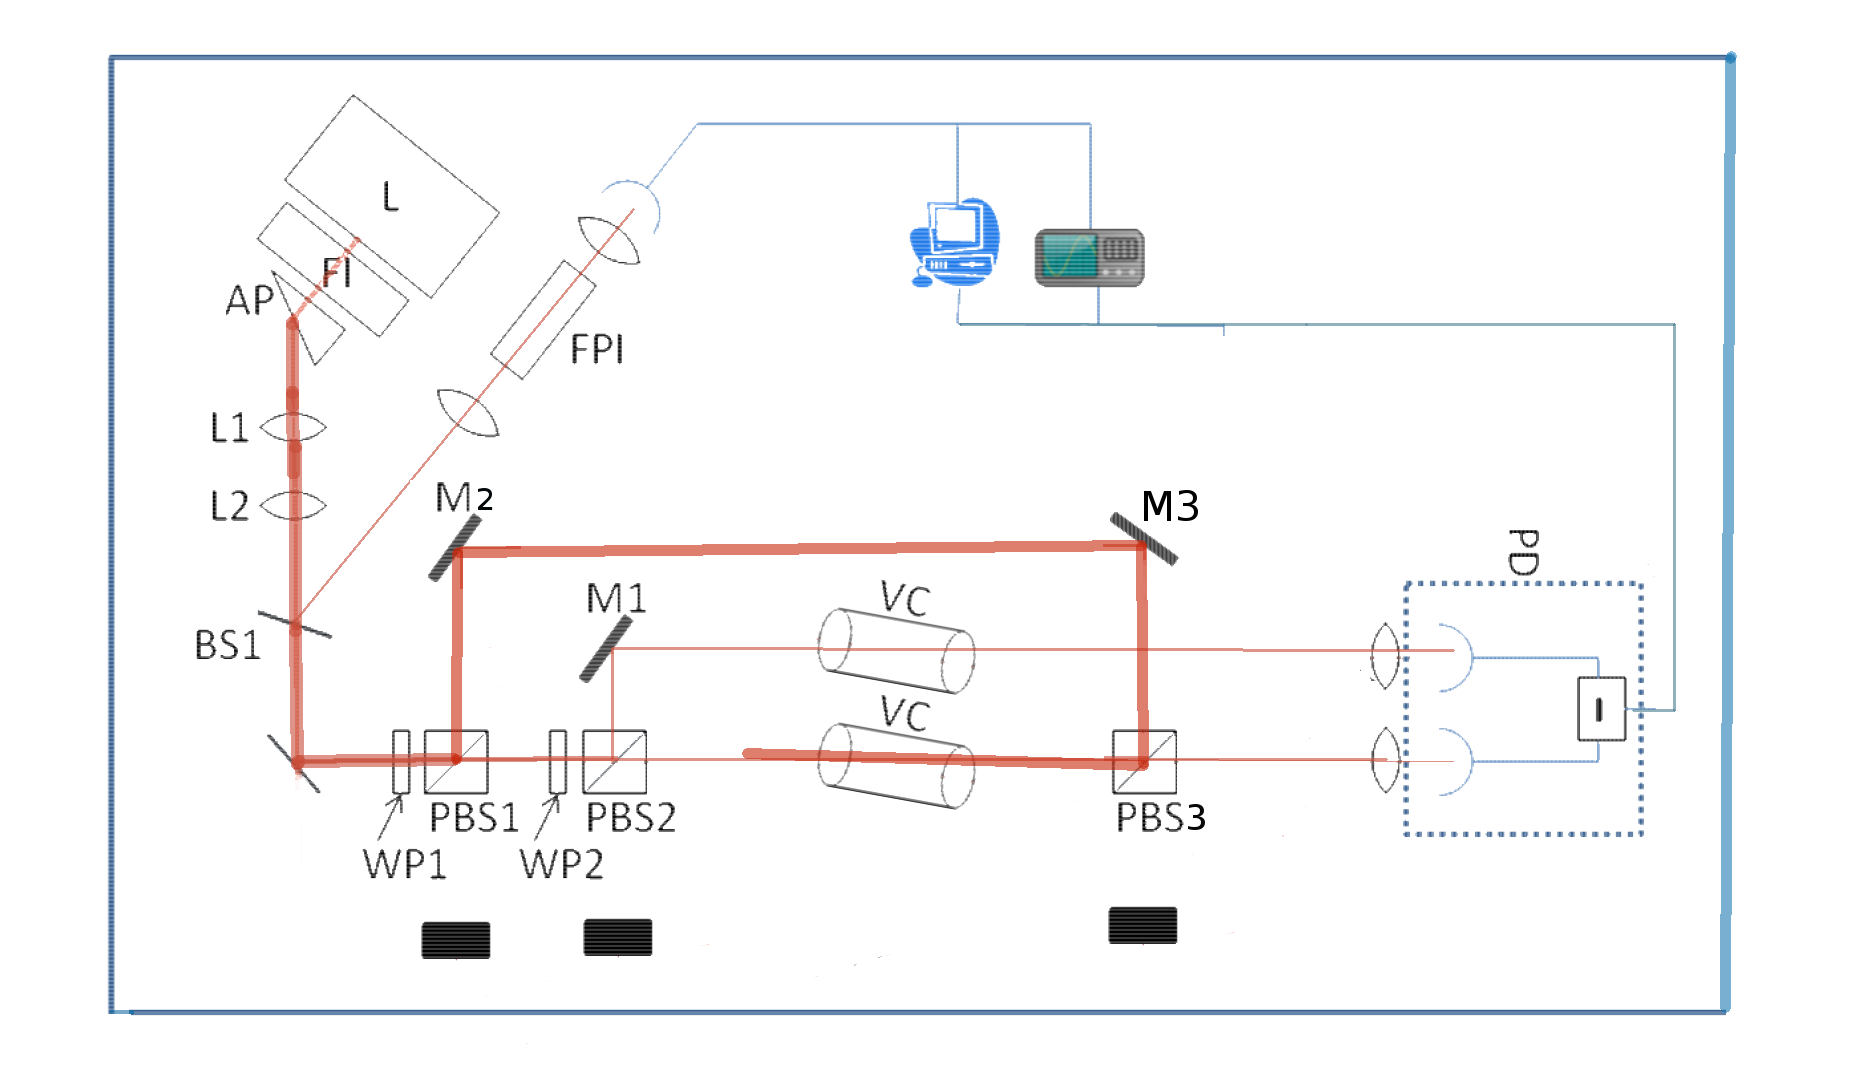
\includegraphics[width=0.85\textwidth]{./Dopplerfrei.png}
  \caption{Schematischer Aufbau der dopplerfreien Spektroskopie}
\end{figure}

Im zweiten Versuchsteil haben wir den selben Aufbau verwendet und etwas modifiziert. 

Anstatt den p-polarisierten Strahl am PBS1 abzublocken, nutzt man die um Gr��enordnungen
h�here Intensit�t als Pumpstrahl. Er soll m�glichst auf der gleichen Geraden wie der Teststrahl durch die Rubidiumzelle 
laufen, um die zu messenden Hyperfeinstrukturlinien zu s�ttigen. 

Daf�r wird der Strahl mit zwei Spiegeln auf PBS3 geworfen, der mittig in die Bahn des Teststrahles zwischen Zelle und Photodiode
positioniert wird. Den Pumpstrahl l�sst er transmittieren oder reflektiert ihn auf die Teststrahlgerade, je nach dem wie er polarisiert ist.

Den Teststrahl l�sst er im Idealfall unber�hrt transmittieren, da er bereits durch PBS2 p-polarisiert ist.

Mit einem weiteren \( \frac{\lambda}{2} \)-Pl�ttchen, das zwischen Spiegel M3 und PBS3 gestellt wird, kann die Intensit�t des Pumpstrahles variiert werden. Dies wird f�r die Messung der S�ttigungsintensit�t ben�tigt.

Da der Transmissionsunterschied zu der vorherigen Messung in den ges�ttigten Hyperfeinstrukturlinien liegt,
ist es sinnvoll eine weitere Rubidiumzelle in den Referenzstrahl zu stellen, um am Oszilloskop die Linien zu sehen.


Nachdem der Aufbau f�r den zweiten Versuchteil justiert wurde und man die erwarteten 3 Hyperfeinstreinstrukterpeaks 
und 3 Crossover-peaks am Oszilloskop sehen kann, f�ngt man mit der Vermessung der Strahlgr��e an.

Zwischen Spiegel M2 und M3 haben wir eine Rasiermesserklinge an einem Ger�st befestigt platziert. Diese kann man 
in den Strahl positionieren, sodass er einen Teil der Leistung des Strahls abh�ngig von seiner Position abf�ngt. 
Hinter der Klinge haben wir die Strahlleistung gemessen und diese zusammen mit der Position in einer Tabelle eingetragen.
Das haben wir jeweils f�r die horizontale und die vertikale Strahlbreite (\(w_x, w_y\)) gemacht, da wir davon ausgingen, dass der
Strahl nicht perfekt kreisf�rmig ist, sondern eventuell leicht elliptisch.


In der n�chsten Messreihe haben wir die Leistung des Pumpstrahls im Bereich von 20 bis 800 \(�\)W variiert 
und die Peaks der 78-F2-Linie am Oszilloskop aufgenommen.

Die Daten haben wir mit Origin verwertet und die nat�rliche Linienbreite und die S�ttigungsintensit�t bestimmt.
